\documentclass{article}
\usepackage[utf8]{inputenc}
\usepackage{amsmath}
\usepackage{mathtools}
\usepackage{graphicx}
\graphicspath{ {./drift/} }
\DeclarePairedDelimiter{\ceil}{\lceil}{\rceil}
\usepackage{geometry}
\usepackage[banglamainfont=Kalpurush, 
            banglattfont=Siyam Rupali
           ]{latexbangla}
        
\begin{document}
\begin{LARGE}
\begin{center}
তাড়ন বেগ ও তড়িৎপ্রবাহ ঘনত্ব
\end{center}
\end{LARGE}
\textbf{তড়িৎপ্রবাহ ঘনত্ব $ J $:} একটি পরিবাহীর প্রতি একক সময় ও ক্ষেত্রফলে মোট যে পরিমাণ চার্জ প্রবাহিত হয় তাকে তড়িৎপ্রবাহ ঘনত্ব $ J $ দ্বারা চিহ্নিত করা হয়।\\
\[ J = \dfrac{\triangle q}{A\triangle t}\]

যেখানে $ \triangle q $ হচ্ছে $ A $ ক্ষেত্রফলের ভিতর দিয়ে $ \triangle t $ সময়ে প্রবাহিত মোট চার্জের পরিমাণ। চিত্রে একটি পরিবাহীর প্রস্থচ্ছেদের ক্ষেত্রফল $ A $ এর ভিতর দিয়ে প্রয়োগকৃত তড়িৎক্ষেত্র $ E_{x} $  উপস্থিতিতে ইলেকট্রনের নেট প্রবাহ দেখানো হয়েছে। লক্ষ্য করলে দেখা যাবে যে, ইলেকট্রনের গতির দিক তড়িৎক্ষেত্র $ E_{x} $ এবং প্রচলিত প্রবাহের উল্টাদিকে কারন, ইলেকট্রনগুলো তাদের ঋণাত্মক চার্জের কারণে $ x $ অক্ষের দিকে একটি কুলম্বিক বল $ eE_{x} $ অনুভব করে।\\

 আমরা জানি, ধাতুর পরমাণুর সঞ্চারণশীল ইলেট্রনগুলো উদ্দেশ্যবিহীনভাবে ঘুরাঘুরি করে কিন্তু একটি তড়িৎক্ষেত্র $ E_{x} $ প্রয়োগ করার ফলে তারা $ x $ অক্ষের দিকে একটি লদ্ধিবেগ অর্জন করে। অন্যথায় $ A $ প্রস্থচ্ছেদের ক্ষেত্রফলের ভিতর দিয়ে ইলেকট্রনগুলো কোন লদ্ধি প্রবাহ অর্জন করতে পারতোনা।
 
 $ x $ অক্ষের দিকে $ t $ সময়ে ইলেকট্রনগুলোর গড় গতিবেগকে $ v_{dx}(t) $ দ্বারা চিহ্নিত করা হয়। একে তাড়নবেগ বলে যা $ x $ অক্ষের দিকে অনেক ইলেকট্রনের (আনুমানিক $ \sim 10^{28} m^{-3} $)  তাৎক্ষণিক বেগ $ v_x $ এর গড়
 \[ v_{dx} = \dfrac{1}{N} [v_{x_{1}} + v_{x_{2}}+ v_{x_{3}}+ \cdots + v_{x_{N}}] \]
 
 
 যেখানে $ v_{x_{i}} $ হচ্ছে $ x $ অক্ষের দিকে $ i $ তম ইলেকট্রনের বেগ এবং $ N $ হচ্ছে ধাতুর পরমাণুর সঞ্চারনশীল ইলেকট্রনের সংখ্যা। ধরা যাক $ n =\dfrac{N}{A}$ হচ্ছে  পরিবাহীর প্রতি একক আয়তনে ইলেকট্রন সংখ্যা। এবং $ \triangle t $ সময়ে ইলেকট্রন $ \triangle x = v_{dx}\triangle t $ পথ অতিক্রম করে। সুতরাং পরিবাহীর প্রচ্ছেদের ক্ষেত্রফল $ A $ তে মোট অতিক্রমকারী চার্জ $ \triangle q = enA\triangle x $ । কারণ $ \triangle x $ দুরত্বের মধ্যে সকল ইলেকট্রন $ A $ ক্ষেত্রফলের ভিতর দিয়ে অতিক্রম করে। সুতরাং $ n(A \triangle x) $ হচ্ছে $ \triangle t $ সময়ে $ A $ ক্ষেত্রফলের ভিতর দিয়ে অতিক্রমকারী চার্জের সংখ্যা। তাহলে $ x $ অক্ষের দিকে তড়িৎপ্রবাহ ঘনত্ব 
 
 \[ J_{x} = \dfrac{\triangle q}{A\triangle t} = \dfrac{enAv_{dx}\triangle t}{A\triangle t} = env_{dx}\]
\begin{center}
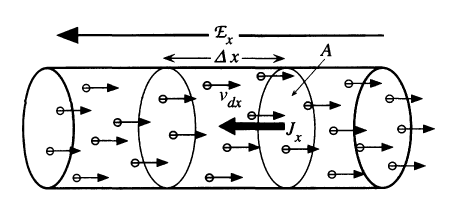
\includegraphics{2018-07-24_072834.png}
\end{center}

উপরোক্ত সাধারন সমীকরণটি $ J_{x} $ এবং ইলেকট্রনের গড়বেগ $  v_{dx} $ এর মধ্যে সম্পর্ক নির্দেশ করে। এটা খুবই সুবিধাজনক যে যেকোন এক সময়ের গড়বেগ অন্যসময়ের গড়বেগের সমান নাও হতে পারে কারন প্রয়োগকৃত তড়িৎক্ষেত্র সময়ের সাপেক্ষ্যে পরিবর্তন হতে পারে যেমন: $ E_{x} = E_{x}(t) $।  তাহলে সময় সাপেক্ষ্য একটি প্রবাহের জন্য লেখা যায়: \[ J_{x} (t)= env_{dx}(t)\]

তড়িৎপ্রবাহ ঘনত্ব $ J_{x} $ এবং তড়িৎক্ষেত্র $ E_{x} $ এর মধ্যে সম্পর্ক স্থাপনের জন্য পরিবাহীর সঞ্চারণশীল ইলেকট্রনের গতির উপর তড়িৎক্ষেত্রের প্রভাব পরীক্ষা করতে হবে। এর জন্য একটি কপার ক্রিস্টালকে বিবেচনা করা যাক।

কপার পরমাণুর $ 4s $ সাবসেলে একটি মাত্র যোজনী ইলেকট্রন থাকে যা খুবই দুর্বলভাবে আবদ্ধ থাকে। Face-centered cubic (FCC) crystal structure-এ কঠিন ধাতু ধনাত্নক আয়ন কোর দ্বারা গঠিত, $ Cu^{+} $। কঠিন ধাতুতে যোজনী ইলেকট্রনগুলো নিজেদের বিচ্ছিন্ন করে মুক্তভাবে ঘুরাঘুরি করে ইলেকট্রন মেঘ বা গ্যাস সৃষ্টি করে। এই সঞ্চারণশীল ইলেকট্রনগুলোই তড়িৎক্ষেত্র দ্বারা সহজে প্রভাবিত হয় এবং তড়িৎপ্রবাহ ঘনত্ব সৃষ্টি করে। ইলেকট্রন গ্যাসে যোজনী ইলেকট্রনগুলোই মুলত পরিবাহী ইলেকট্রন।\\

ঋনাত্বক ইলেকট্রন মেঘ এবং $ Cu^{+} $ আয়নের আকর্ষণী বলই মুলত ধাতব বন্ধন ও কঠিন ধাতুর জন্য দ্বায়ী। পরিবাহী ইলেকট্রন ও ধাতুর ধনাত্নক আয়নের স্থিরবৈদ্যুতিক আকর্ষণ, হাইড্রাজেন পরমাণুর ইলেট্রন ও প্রোটনের মধ্যকার স্থিরবৈদ্যুতিক আকর্ষণের মত যা পরিবাহী ইলেকট্রনকে স্থিতি শক্তি ও গতিশক্তি প্রদান করে। একটি গ্যাসীয় পরমানু একটি সিলিন্ডারে যেমনভাবে চলাচল করে ঠিক একইভাবে পরিবাহী ইলেকট্রনগুলো একটি ক্রিস্টাল ল্যাটিসে ঘুরাফেরা করে। যদিও গ্যাসীয় পরমাণুর গড় গতিশক্তি $ \frac{3}{2}KT $ যা ইলেকট্রনের জন্য প্রযোজ্য নয় কারণ ইলেট্রনগুলো ধাতব আয়নের সাথে স্থির বৈদ্যিুতিক আকর্ষনের কারনে শক্তিশালী ক্রিয়াশীলতা প্রদর্শন করে।\\

প্রাথমিকভাবে ইলেকট্রনের গড় গতিশক্তি নির্ণয় করা হয় ধনাত্নক ধাতব আয়ন ও ইলেকট্রনের মধ্যকার স্থির বৈদ্যুতিক ক্রিয়াশীলতা থেকে। আরও বাস্ততভাবে বুঝার জন্য গড় গতিশক্তির তাপমাত্রা নির্ভরশীলতাকে যে অন্যান্য অনেক ফ্যাক্টরের সাথে তুলনা করা হয় যারা ধাতুর ক্রিস্টালে পরিবাহী ইলেকট্রনের আচরণ নিয়ন্ত্রন করে সেগুলোকে অগ্রাহ্য করা হয়।



\end{document}